\documentclass{article}

\usepackage[normalem]{ulem}
\usepackage{fancyhdr}
\usepackage[parfill]{parskip}
\usepackage{tikz}
\usepackage{multicol}
\usepackage{makecell}
\usepackage{multirow}
\pagestyle{fancyplain}
\usetikzlibrary{shapes, patterns, arrows}

\title{Respiration}
\author{Todd Davies}
\date{\today}

\begin{document}

\rhead{Respiration}
\lhead{\today}

\maketitle

\section*{The stages of respiration}
\thispagestyle{empty}
Respiration releases the energy stored in glucose by oxidising it and creates ATP.

There are four stages of respiration, glycolysis, the link reaction, the Krebs cycle, and the electron transport chain.

\subsection*{Glycolysis}
Gylcolysis takes place in the cytoplasm of the cell. It can function without oxygen.

Since sugars are unreactive, two molecules of ATP are used to add two phosphate groups to the glucose molecule, which is then broken down into two molecules of TP (triose phospoate). The TP is then oxidised to pyruvate and reduced NAD. This releases enough energy to create four ATP molecules from four ATP + pi molecules.

Since two ATP molecules were used to start the reaction, there is a \textbf{net gain of two ATP} molecules.

Here is a diagram of glycolysis:

\begin{center}
	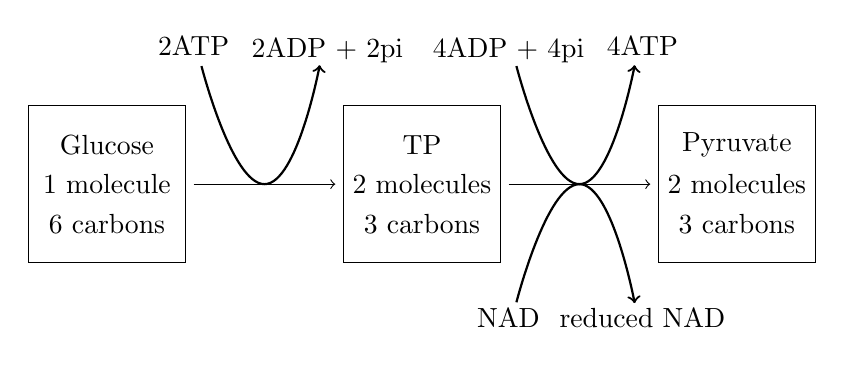
\begin{tikzpicture}
	%Glucose
		\draw (0,0) rectangle (2,2);
		\node at (1,1.5) {Glucose};
		\node at (1,  1) {1 molecule};
		\node at (1,0.5) {6 carbons};
	%Glucose->TP
		\draw[->] (2.1,1) -- (3.9,1);
	%ATP->ADP + pi
		\draw[thick] plot [smooth,tension=1] coordinates{(2.2, 2.5) (3, 1) (3.7, 2.5)};
		\draw [thick, ->] (3.7, 2.5) -- (3.701, 2.51);   %Right
		\node at (2.1, 2.75) {2ATP};
		\node at (3.8, 2.7) {2ADP + 2pi};
	%TP
		\draw (4,0) rectangle (6,2);
		\node at (5,1.5) {TP};
		\node at (5,  1) {2 molecules};
		\node at (5,0.5) {3 carbons};
	%TP->Pyruvate
		\draw[->] (6.1,1) -- (7.9,1);
	%ADP+pi->ATP
		\draw[thick] plot [smooth,tension=1] coordinates{(6.2, 2.5) (7, 1) (7.7, 2.5)};
		\draw [thick, ->] (7.7, 2.5) -- (7.701, 2.51);   %Right
		\node at (6.1, 2.7) {4ADP + 4pi};
		\node at (7.8, 2.75) {4ATP};
	%NAD->reduced NAD
		\draw[thick] plot [smooth,tension=1] coordinates{(6.2, -0.5) (7, 1) (7.7, -0.5)};
		\draw [thick, ->] (7.7, -0.5) -- (7.701, -0.51);   %Right
		\node at (6.1, -0.7) {NAD};
		\node at (7.8, -0.7) {reduced NAD};
	%Pyruvate
		\draw (8,0) rectangle (10,2);
		\node at (9,1.5) {Pyruvate};
		\node at (9,  1) {2 molecules};
		\node at (9,0.5) {3 carbons};
	\end{tikzpicture}
\end{center}

The arrow between glucose and TP describes phosphorylation, and the arrow between TP and pyruvate represents oxidation.

\subsection*{The link reaction}
Takes place in the mitochondria.

First, pyruvate from glycolysis enters the mirochondria, where NAD removes electrons from the pyruvate, oxidising it into acetylcoenzyme A and carbon dioxide. This reaction is termed \textbf{oxidative decarboxylation}.

Here is a diagram of the link reaction:

\begin{center}
	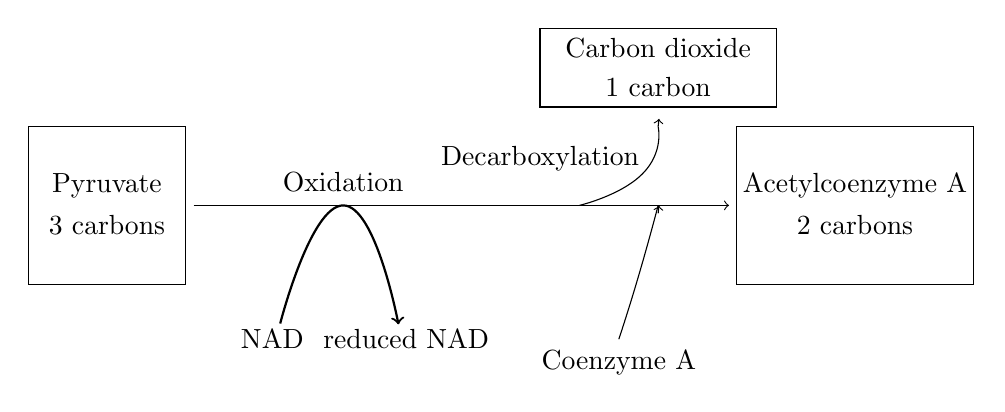
\begin{tikzpicture}
	%Pyruvate
		\draw (0,0) rectangle (2,2);
		\node at (1,1.25) {Pyruvate};
		\node at (1,0.75) {3 carbons};
	%Pyruvate->Acetylcoenzyme A
		\draw[->] (2.1,1) -- (8.9,1);
	%Oxidation
		\node at (4, 1.3) {Oxidation};
	%NAD->reduced NAD
		\draw[thick] plot [smooth,tension=1] coordinates{(3.2, -0.5) (4, 1) (4.7, -0.5)};
		\draw [thick, ->] (4.7, -0.5) -- (4.701, -0.51);   %Right
		\node at (3.1, -0.7) {NAD};
		\node at (4.8, -0.7) {reduced NAD};
	%Decarboxylation
		\draw plot [smooth,tension=1] coordinates{(7, 1) (7.8, 1.4) (8, 2)};
		\draw [->] (8, 2) -- (8.01, 2.1);   %Right
		\node at (6.5, 1.6) {Decarboxylation};
	%Coenzyme A
		\draw plot [smooth,tension=1] coordinates{(7.5, -0.7) (7.75, 0.1) (8, 1)};
		\draw [->] (8, 0.9) -- (8.01, 1);   %Right
		\node at (7.5, -1) {Coenzyme A};
	%Carbon dioxide
		\draw (6.5,2.25) rectangle (9.5,3.25);
		\node at (8,3) {Carbon dioxide};
		\node at (8,2.5) {1 carbon};
	%Acetylcoenzyme A
		\draw (9,0) rectangle (12,2);
		\node at (10.5,1.25) {Acetylcoenzyme A};
		\node at (10.5,0.75) {2 carbons};
	\end{tikzpicture}
\end{center}

\textit{N.b since each glucose molecule produces two pyruvate molecules in glycolysis, the link reaction runs twice for every one glucose molecule respired.}

\subsection*{Krebs cycle}
Occurs in the matrix of the mitochondria. The aim of the Krebs cycle is to supply electrons to the electron transport chain, so it doesn't directly create very much ATP.

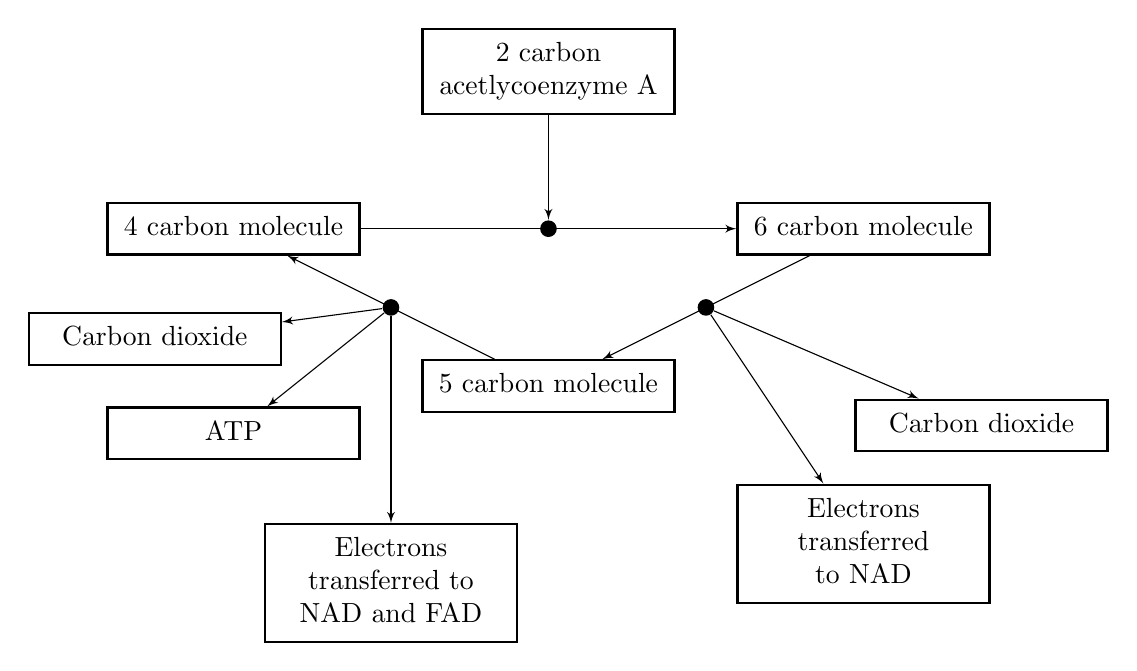
\begin{tikzpicture}

	% Define block styles
	\tikzstyle{line} = [draw, -latex']
	\tikzstyle{connector} = [fill,circle,inner sep=0pt,minimum size=6pt]


	\node[thick,draw,minimum height=0.5cm,minimum width=3.2cm] (acetylcoenzymeA) at (0,0) {\makecell[c]{2 carbon\\acetlycoenzyme A}};
	
	\node[connector] (center) at (0, -2) {};
	
	\node[thick,draw,minimum height=0.5cm,minimum width=3.2cm] (6C) at (4,-2) {\makecell[c]{6 carbon molecule}};
	
	\node[connector] (6-5) at (2, -3) {};
	
	\node[thick,draw,minimum height=0.5cm,minimum width=3.2cm] (5C) at (0,-4) {\makecell[c]{5 carbon molecule}};
	
	\node[connector] (5-4) at (-2, -3) {};
	
	\node[thick,draw,minimum height=0.5cm,minimum width=3.2cm] (4C) at (-4,-2) {\makecell[c]{4 carbon molecule}};
	
	\node[thick,draw,minimum height=0.5cm,minimum width=3.2cm] (1_CO2) at (5.5,-4.5) {\makecell[c]{Carbon dioxide}};
	
	\node[thick,draw,minimum height=0.5cm,minimum width=3.2cm] (electrons_to_NAD) at (4,-6) {\makecell[c]{Electrons \\transferred\\to NAD}};
	
	\node[thick,draw,minimum height=0.5cm,minimum width=3.2cm] (2_CO2) at (-5,-3.4) {\makecell[c]{Carbon dioxide}};
	
	\node[thick,draw,minimum height=0.5cm,minimum width=3.2cm] (ATP) at (-4,-4.6) {\makecell[c]{ATP}};
	
	\node[thick,draw,minimum height=0.5cm,minimum width=3.2cm] (electrons_to_NAD_FAD) at (-2,-6.5) {\makecell[c]{Electrons \\transferred to\\NAD and FAD}};

	\path [line] (acetylcoenzymeA) -- (center);
	\path [line] (4C) -- (6C);
	\path [line] (6C) -- (5C);
	\path [line] (5C) -- (4C);
	\path [line] (6-5) -- (1_CO2);
	\path [line] (6-5) -- (electrons_to_NAD);
	\path [line] (5-4) -- (2_CO2);
	\path [line] (5-4) -- (ATP);
	\path [line] (5-4) -- (electrons_to_NAD_FAD);
\end{tikzpicture}

\subsection*{Electron transport chain}
It is here that most of the ATP is created for respiration.

Here are the steps:
\begin{enumerate}
	\item The reduced FAD and NAD release their hydrogen atoms as they are oxidised to FAD and NAD. These hydrogen atoms split into protons and electrons.
	\item The electrons move along the electron transport chain and lose energy as they do so. This energy is used to pump protons from the mitochondrial matrix into the intermembrane space (between the inner and outer mitochondrial membranes).
	\item This creates a concentration gradient of protons (more in intermembrane space).
	\item The protons move back into the matrix of the mitochondrion by passing through ATPase. This provides the energy to synthesise ATP from ADP + pi.
	\item The protons, electrons and oxygen combine to form water.
\end{enumerate}

\textit{N.b. the movement of $H^+$ ions across a membrane is called chemiosmosis.}

\section*{The amount of ATP produced}
This table shows the amount of ATP produced for one glucose molecule respired:

\begin{center}
	\begin{tabular}{|l|l|r|}
		\hline
			Stage & Molecules made & \# ATP produced\\ \hline
			Glycolysis & 2 ATP & 2\\ \hline
			Glycolysis & 2 reduced NAD & $2 \times 2.5 = 5$\\ \hline
			Link reaction ($\times 2$) & 2 reduced NAD & $2 \times 2.5 = 5$\\ \hline
			Krebs cycle ($\times 2$) & 2 ATP & 2\\ \hline
			Krebs cycle ($\times 2$) & 6 reduced NAD & $6 \times 2.5 = 15$\\ \hline
			Krebs cycle ($\times 2$) & 2 reduced FAD & $2 \times 1.5 = 3$\\ \hline
			\multicolumn{3}{|r|}{Total ATP = 32}\\ \hline
	\end{tabular}
\end{center}

Research shows that one molecule of reduced FAD can produce 1.5 ATP molecules and one molecule of reduced NAD can produce 2.5 ATP molecules. We also must take into account that the link reaction and Krebs cycle both run twice per glucose molecule.

\section*{Anaerobic respiration}
When there isn't oxygen available for respiration, anaerobic respiration can be used to supply a little bit of ATP just to keep things ticking over. In anaerobic respiration, pyruvate from the link reaction is converted to ethanol (in plants/yeast) or lactate (in mammals/some bacteria). This produces NAD from reduced NAD which means glycolysis can continue to produce a little bit of ATP even though there's no oxygen available.

\section*{Questions to practice}
\textbf{Question 1}\\
Where does the Krebs cycle occur?

\textbf{Answer}\\
The matrix of the mitochondria.

\textbf{Question 2}\\
Carbon monoxide inhibits the production of water in the electron transport chain. Why does this affect ATP production in the electron transport chain and Krebs cycle.

\textbf{Answer}\\
Stops the transfer of electrons through the electron transfer chain (no electrons are taken out) so $H^+$ ions aren't pumped across the membrane and ATPase stops producing ATP.

No NAD and FAD are produced by the electron transfer chain and so the Krebs cycle cannot continue (since it has nowhere to offload extra electrons).

\textbf{Question 3}\\
Describe how glucose is converted to pyruvate.

\textbf{Answer}\\
In glycolysis, glucose first undergoes phosphorylation by adding two phosphate groups from two ATP molecules which produces two molecules of TP and two molecules of ADP. The TP is then oxidised using electrons from NAD to produce two pyruvate molecules. There is a net gain of 2ATP (2 used, 4 made).

\textbf{Question 4}\\
Write an equation to show how lactate is produced.

\textbf{Answer}\\
\[
	Glucose + ATP \rightarrow 2(TP + ADP) \rightarrow 2 \times pyruvate + \textrm{\textit{reduced NAD}} \rightarrow lactate + NAD
\]

\textbf{Question 5}\\
Why is lactate produced even though no ATP is produced from the reaction?

\textbf{Answer}\\
Reduced NAD is oxidised to NAD which allows glycolysis to continue under anaerobic conditions and produce some ATP.

\end{document}